\subsection{Prompting through first-person demonstrations}
\label{app:prompting}

Figure \ref{fig:prompting-all-tasks} shows the performance of AdA prompted with a fine-tuned agent compared to an unprompted baseline on each of the 30 single agent hand-authored probe tasks. The figure reveals a set of tasks on which AdA is able to leverage information in the prompt, resulting in perfect or near perfect scores. There are also tasks where AdA does not seem to be able to do this. In all but one case, prompting does not hurt performance.

\begin{figure}[t]
    \centering
    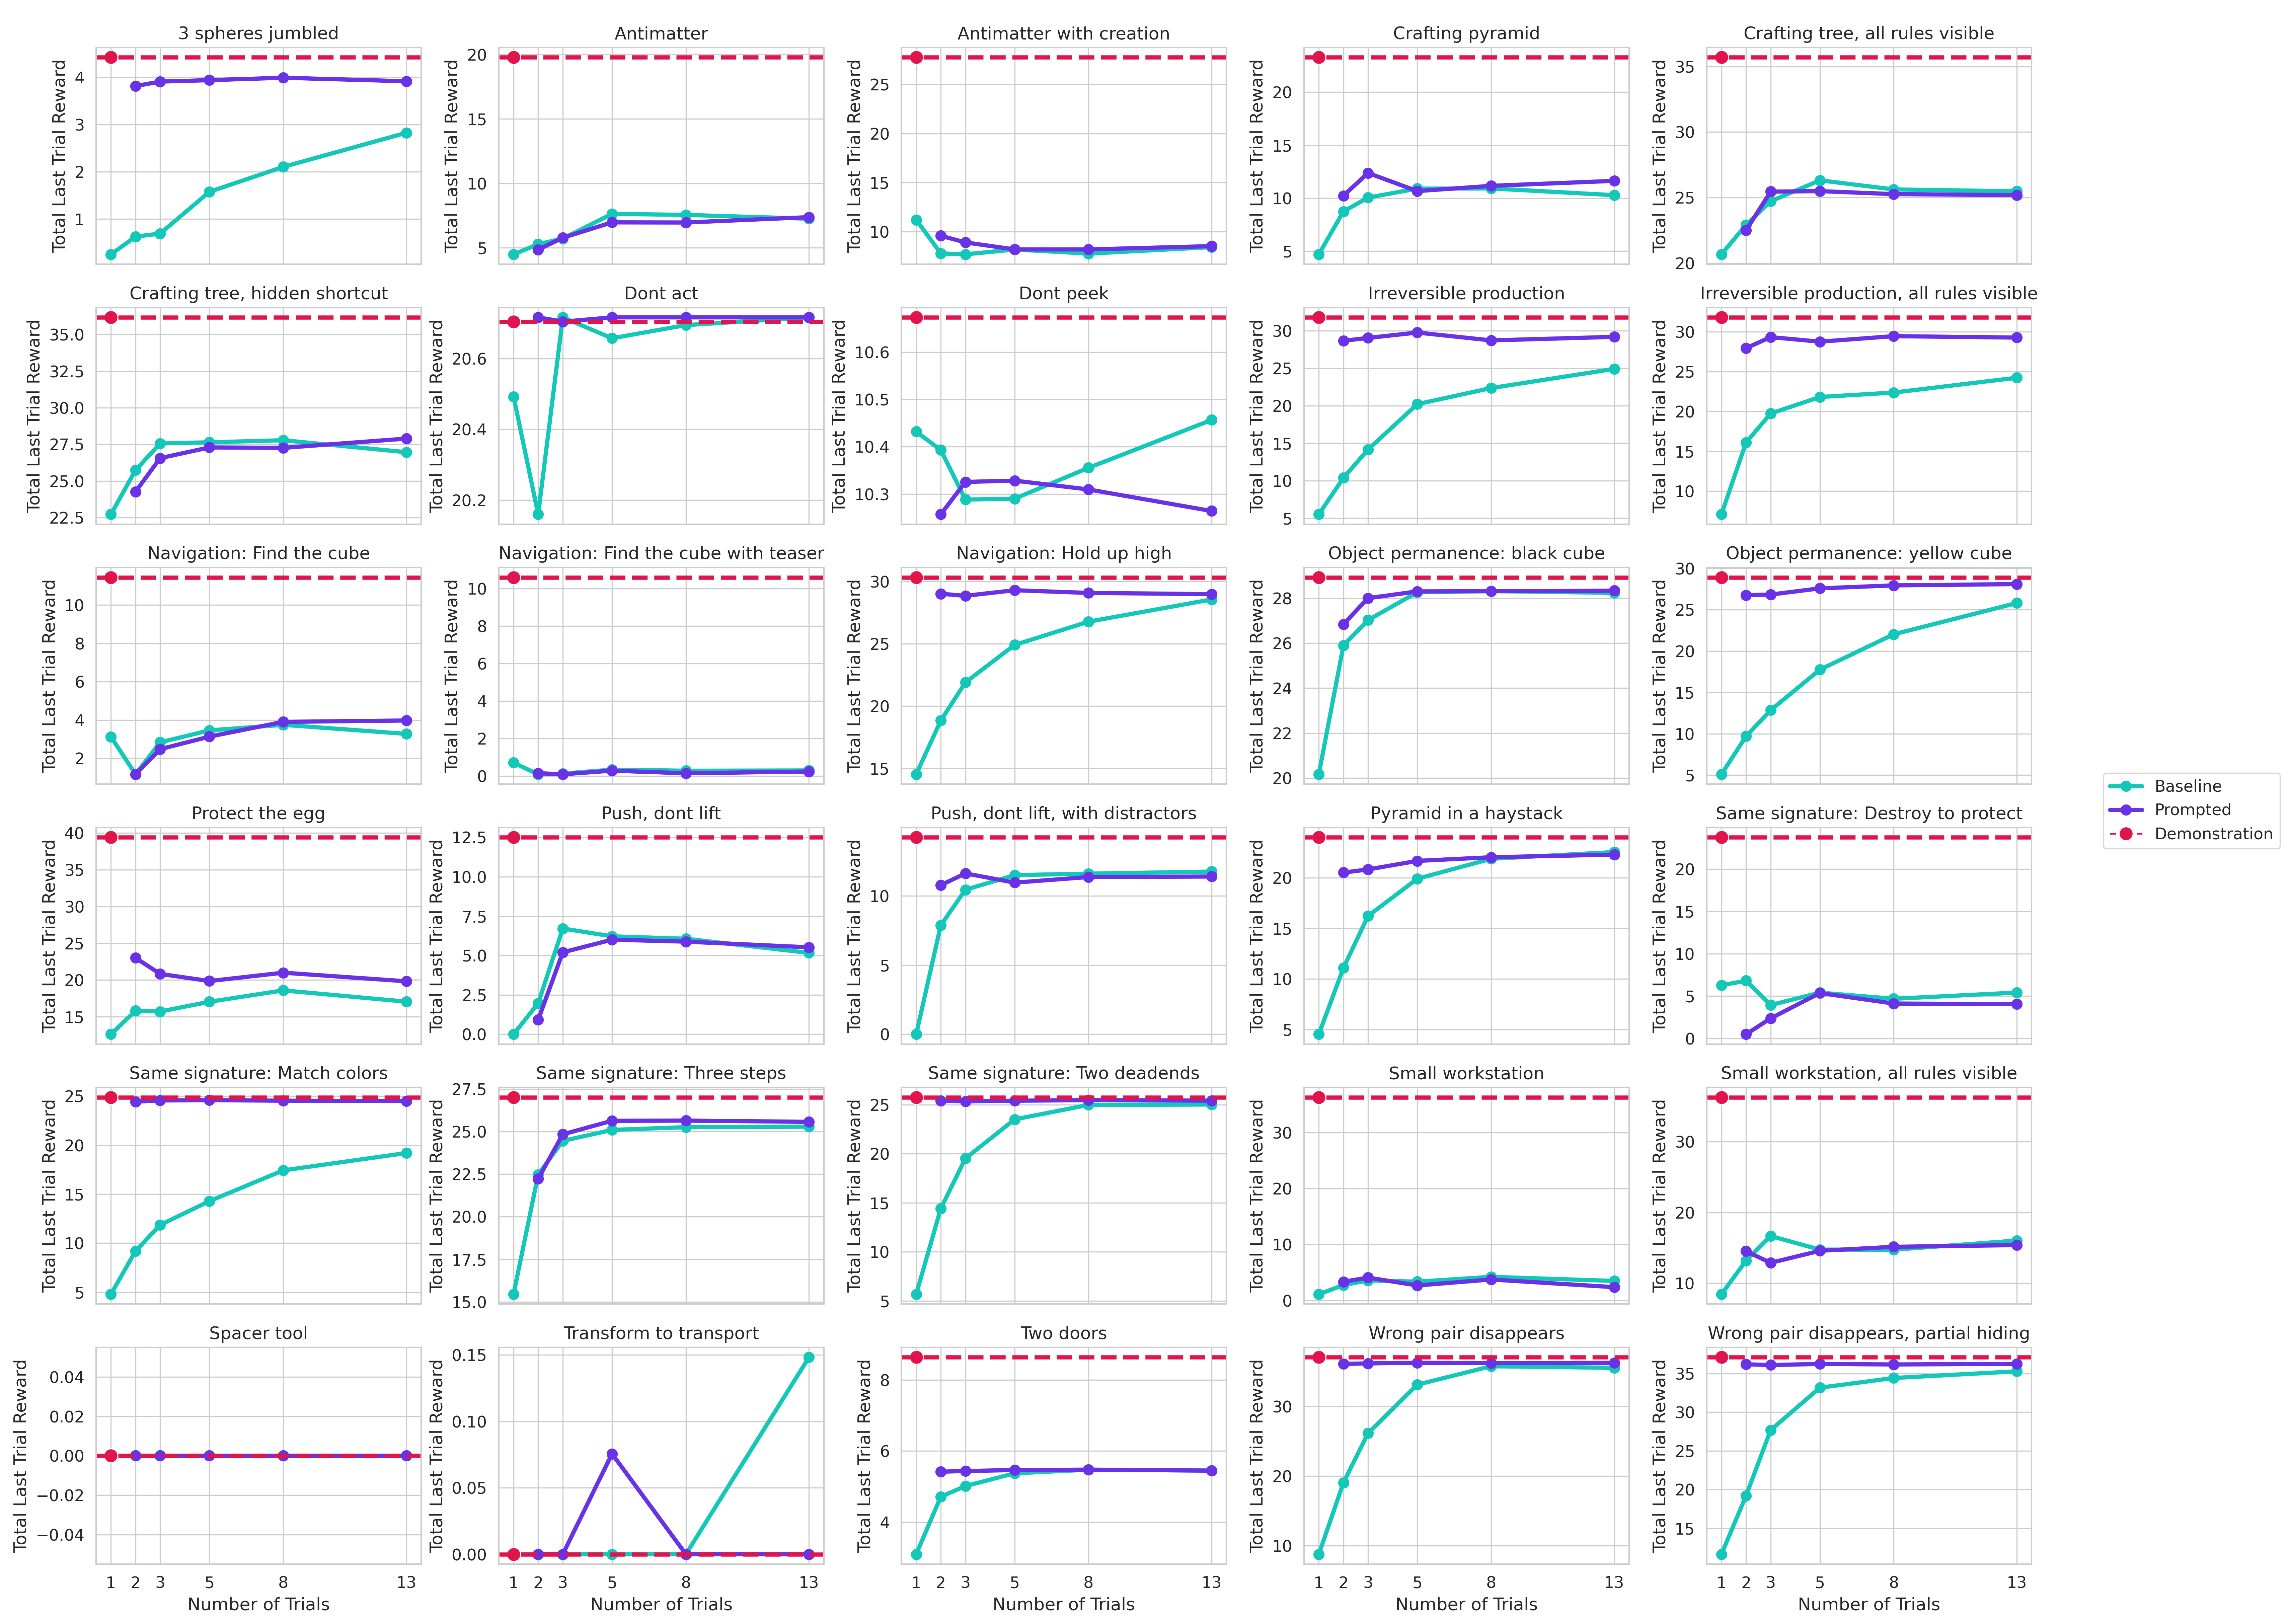
\includegraphics[width=1\linewidth]{figures/prompting-all_tasks.png}
    \caption{A comparison of a prompted agent and unprompted baseline for our full set of 30 hand-authored single-agent tasks. The dashed red lines indicate the score obtained by the teacher providing the first-person demonstration to the prompted agent in the first trial.}
    \label{fig:prompting-all-tasks}
\end{figure}

Analysing the tasks in Figure \ref{fig:prompting-all-tasks} suggests that prompting is useful for short navigational tasks such as \texttt{Navigation: hold up high} in which the agent follows a short and simple path to reach the goal object. Prompting does not, however, improve performance for longer and more complex navigation tasks like \texttt{Navigation: find the cube}, likely due to the full demonstration being too long to fit in the agent’s memory context.

We observe a similar pattern in tasks involving production rules. For tasks with up to 2 production rules in the solution path, such as \texttt{Same signature: match colors}, we observe the unprompted agent exploring different objects to determine the correct rule to trigger. When prompted with a demonstration it subsequently triggers the correct rule immediately and achieves a perfect score. An exception to this is \texttt{Same signature: destroy to protect} where one of the production rules involves destroying an object, which the agent does not appear to remember from the demonstration. For tasks using 3 or more production rules like \texttt{Same signature: three steps} (3 production rules in the solution path) and \texttt{Small workstation} (5 production rules), the agent tends to only remember a subset of the rules to trigger and continues engaging in exploratory behaviour following the demonstration. The performance on these tasks tend to match the unprompted baseline.

Another factor appearing to influence the effectiveness of prompting is the topology and configuration of objects in the world, as seen in the \texttt{Small workstation} tasks. While the teacher demonstrations for these tasks present a clean trajectory, the agent subsequently knocks into and displaces distractor objects, leading to environment states not observed during the demonstration (and thus not recallable from memory). On the other hand, a favourable configuration of objects appears to make the demonstration easier to learn from, as observed in \texttt{Irreversible production}. Here the objects required to trigger the last production rule are positioned close together. The agent shows optimal behaviour here despite the task requiring 3 production rules on the solution path. The agent also appears unable to infer from prompting certain more subtle requirements like relative positioning of objects or tool use. This is observed in tasks like \texttt{Antimatter} in which prompted AdA is able to trigger the destruction rule but we did not observe it immediately hiding objects from each other. 

Prompting may also help eliminate biases that the agent may have acquired during training. This is reflected in the lower score obtained by the unprompted agent for small $k$ in \texttt{Object permanence: yellow cube} compared to \texttt{Object permanence: black cube}. These tasks are identical except for the goal being to navigate to a yellow cube on the right, or a black cube on the left respectively. This suggests that the agent may have acquired a bias during training to either prefer black cubes or to navigate towards objects on its left. The significantly higher prompted scores on \texttt{Object permanence: yellow cube} for small $k$ suggest that a prompt may help the agent overcome these biases.

\begin{figure}[t!]
    \centering
    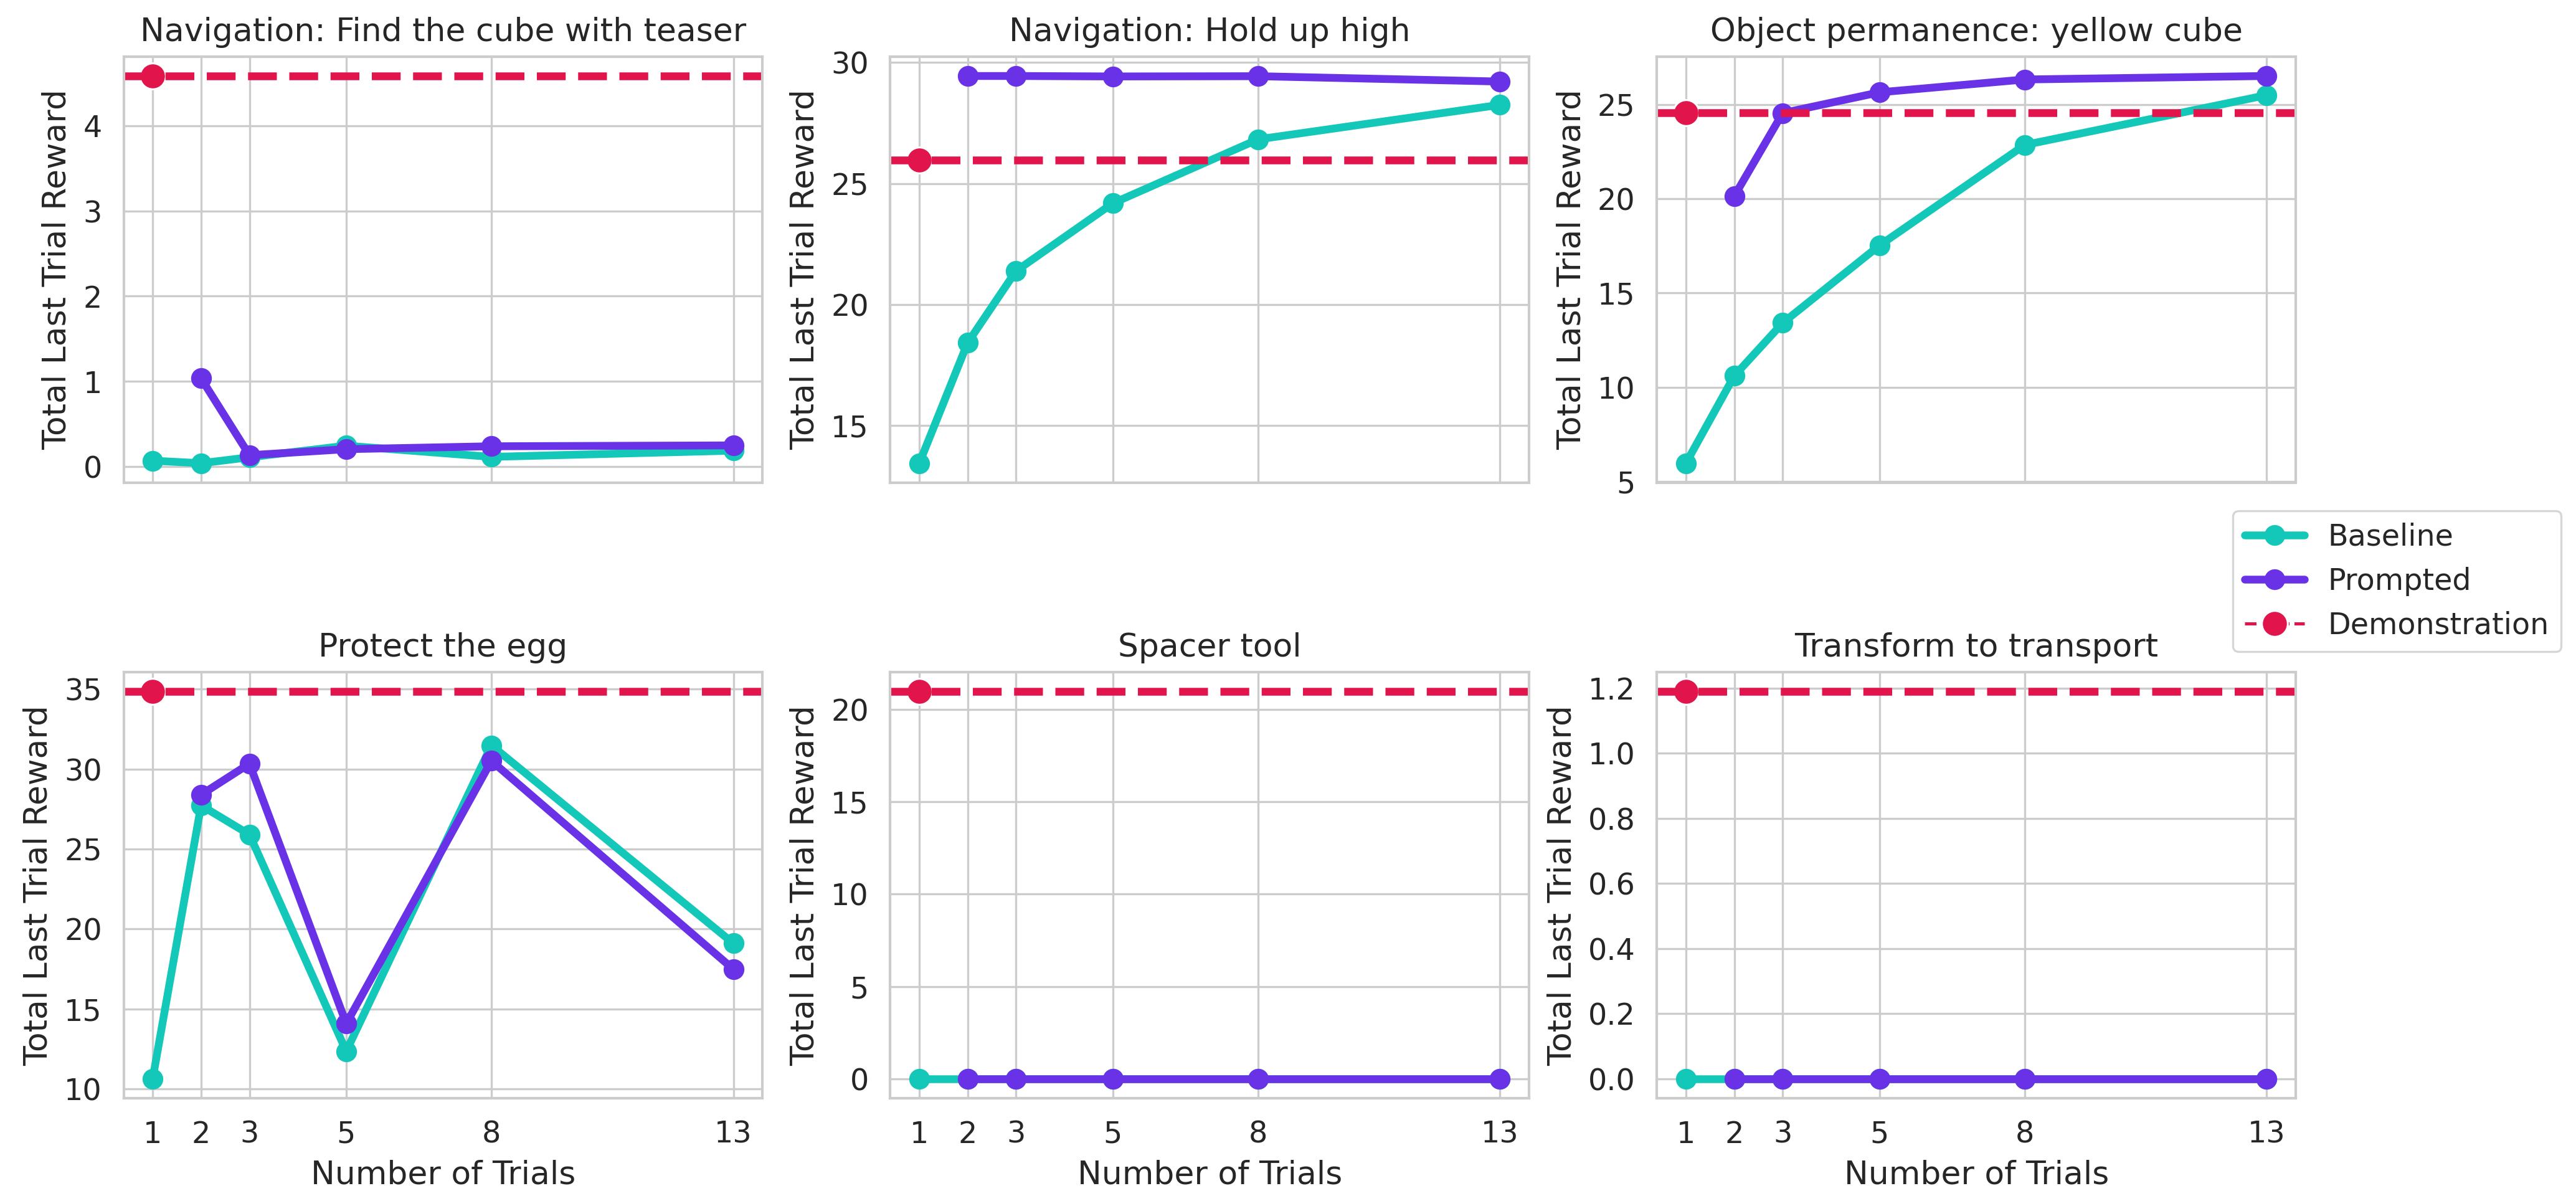
\includegraphics[width=1\linewidth]{figures/human_data_teacher_demo.png}
    \caption{Performance of AdA on 6 hand-authored tasks when prompted with an expert first-person human demonstration, compared with an unprompted baseline.}
    \label{fig:prompting-with-humans}
\end{figure}

\begin{figure}[t!]
    \centering
    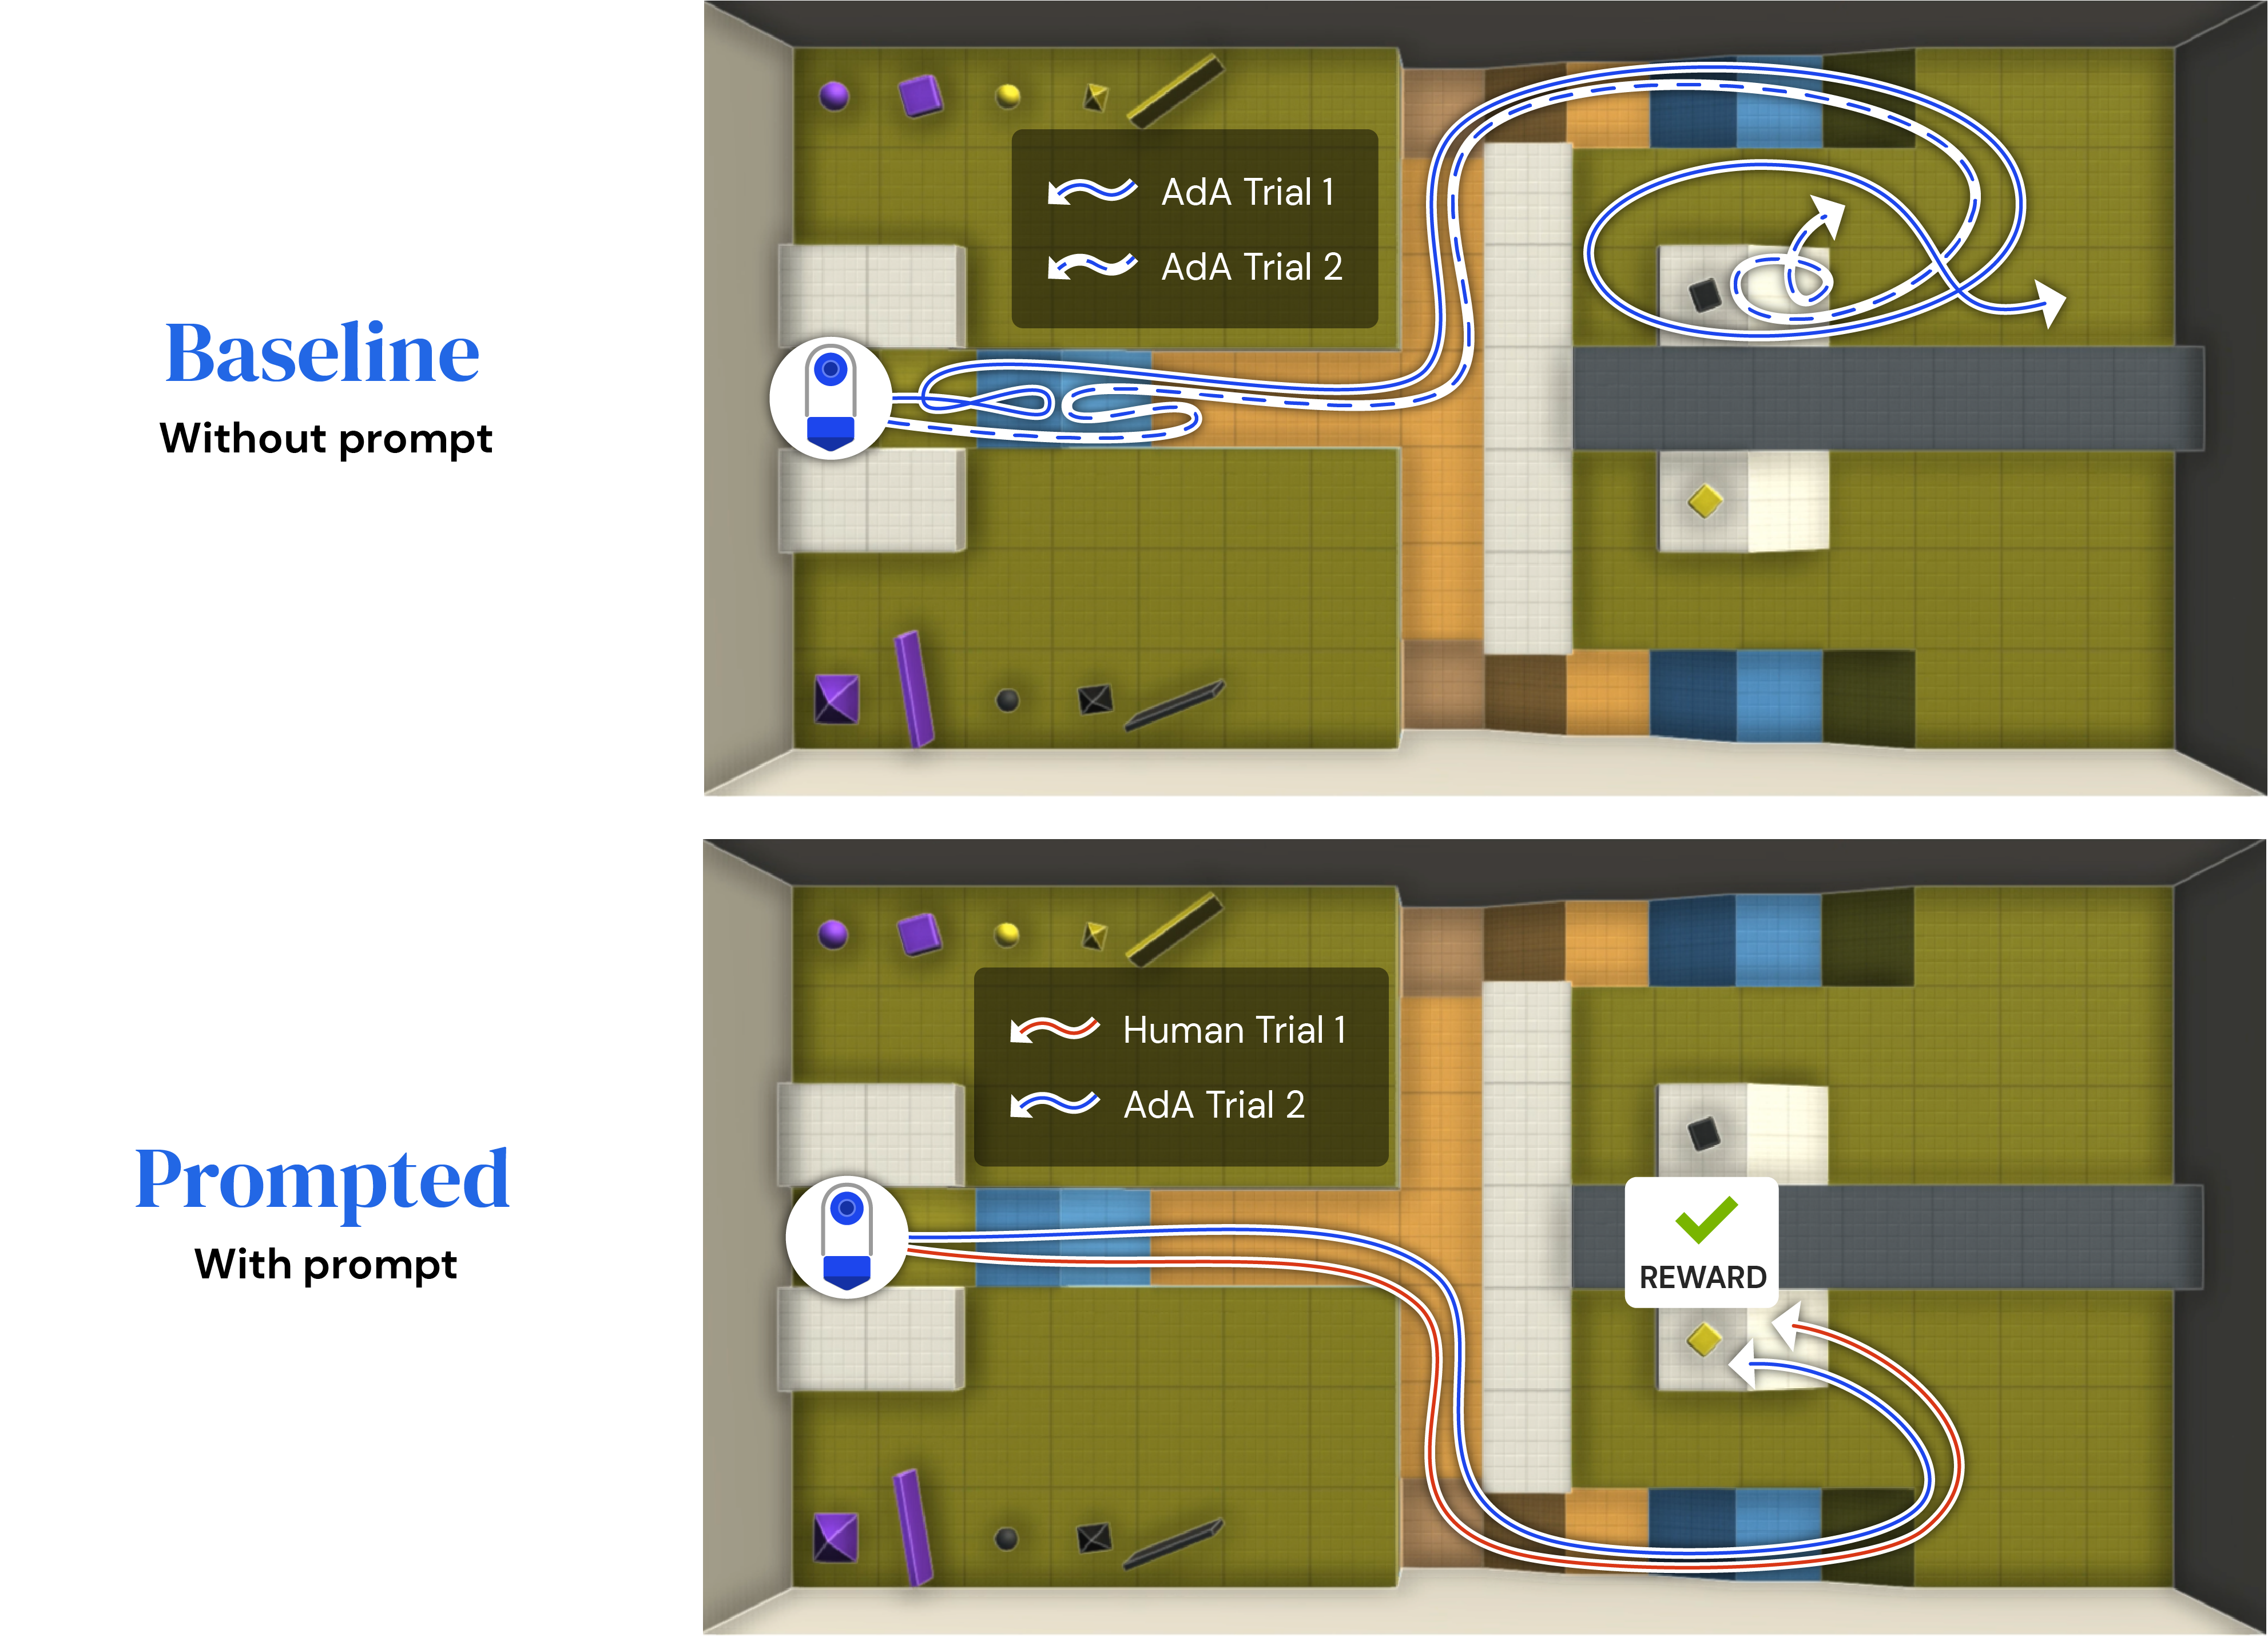
\includegraphics[width=0.6\linewidth]{figures/tasks/trajectories/trajectories_prompt.png}
    \caption{Top-down views depicting the behaviour of AdA with and without a human expert prompt on the task \texttt{Object permanence: yellow cube}. On its own, AdA appears to have a bias of navigating to the black cube which is a dead end in this task. When prompted with a human (or fine-tuned) expert trajectory, AdA is able to overcome this bias and navigate to the yellow cube in the second trial.}
    \label{fig:prompting-trajectory}
\end{figure}

\paragraph{Prompting with human demonstrations.} We prompted AdA with expert human demonstrations in a small selection of 6 hand-authored tasks, depicted in Figure \ref{fig:prompting-with-humans}. These tasks were chosen to be a mixture of tasks where AdA excelled with fine-tuned teacher prompting, where it failed with fine-tuned teacher prompting and where even the fine-tuned teacher failed. 

The results show the same pattern as those obtained when prompting with a fine-tuned teacher. In both \texttt{Navigation: hold up high} and \texttt{Object permanence: yellow cube}, prompted AdA achieved close to optimal performance, exceeding both the baseline and the human demonstration. Figure \ref{fig:prompting-trajectory} depicts the latter behaviour in detail. AdA continues to fail to learn from a demonstration in \texttt{Navigation: find the cube with teaser} and in both \texttt{Spacer tool} and \texttt{Transform to transport}, which our fine-tuned teacher also failed at. A successful human demonstration did not unlock any capabilities AdA was previously not capable of demonstrating, suggesting that these tasks are perhaps too far out-of-distribution with respect to AdA's training tasks. The fact that prompting with off-policy human demonstrations is partially successful is worthy of note, and opens an exciting area of future research. 